% Definiciones y constantes de estilo
% Clase del documento
\documentclass[a4paper, 12pt, twoside, openright, titlepage]{book}

%
% Paquetes necesarios
%

% Símbolo del euro
\usepackage{eurosym}
% Codificación UTF8
\usepackage[utf8]{inputenc}
% Caracteres del español
\usepackage[spanish]{babel}
% Código, algoritmos, etc.
\usepackage{listings}
% Definición de colores
\usepackage{color}
% Extensión del paquete color
\usepackage[table,xcdraw]{xcolor}
% Márgenes
\usepackage{anysize}
% Cabecera y pie de página
\usepackage{fancyhdr}
% Estilo título capítulos
\usepackage{quotchap}
% Algoritmos (expresarlos mejor)
\usepackage{algorithmic}
% Títulos de secciones
\usepackage{titlesec}
% Fórmulas matemáticas
\usepackage[cmex10]{amsmath}
% Enumeraciones
\usepackage{enumerate}
% Páginas en blanco
\usepackage{emptypage}
% Separación entre cajas
\usepackage{float}
% Imágenes
\usepackage[pdftex]{graphicx}
% Mejora de las tablas
\usepackage{array}
% Mejora de los símbolos matemáticos
\usepackage{mdwmath}
% Separar figuras en subfiguras
\usepackage[caption=false,font=footnotesize]{subfig}
% Incluir pdfs externos
\usepackage{pdfpages}
% Mejoras sobre las cajas
\usepackage{fancybox}
% Apéndices
\usepackage{appendix}
% Marcadores (para el pdf)
\usepackage{bookmark}
% Estilo de enumeraciones
\usepackage{enumitem}
% Espacio entre líneas y párrafos
\usepackage{setspace}
% Glosario/Acrónimos
\usepackage[acronym]{glossaries}
% Fuentes
\usepackage[T1]{fontenc}
% Bibliografía
\usepackage[sorting=none,natbib=true,backend=biber,bibencoding=ascii]{biblatex}
% Fix biblatex+babel warning
\usepackage{csquotes}
% debug
\usepackage{etoolbox}

\usepackage{datetime2}

\pdfminorversion=7

\DeclareBibliographyDriver{standard}{%
  \usebibmacro{bibindex}%
  \usebibmacro{begentry}%
  \usebibmacro{author}%
  \setunit{\labelnamepunct}\newblock
  \usebibmacro{title}%
  \newunit\newblock
  \printfield{number}%
  \setunit{\addspace}\newblock
  \printfield[parens]{type}%
  \newunit\newblock
  \usebibmacro{location+date}%
  \newunit\newblock
  \iftoggle{bbx:url}
    {\usebibmacro{url+urldate}}
    {}%
  \newunit\newblock
  \usebibmacro{addendum+pubstate}%
  \setunit{\bibpagerefpunct}\newblock
  \usebibmacro{pageref}%
  \newunit\newblock
  \usebibmacro{related}%
  \usebibmacro{finentry}}



% Enlaces
\hypersetup{hidelinks,pageanchor=true,colorlinks,citecolor=Fuchsia,urlcolor=black,linkcolor=Cerulean}

% Euro (€)
\DeclareUnicodeCharacter{20AC}{\euro}

% Inclusión de gráficos
\graphicspath{{./graphics/}}

% Texto referencias
\addto{\captionsspanish}{\renewcommand{\bibname}{Bibliografía}}

% Extensiones de gráficos
\DeclareGraphicsExtensions{.pdf,.jpeg,.jpg,.png}

% Definiciones de colores (para hidelinks)
\definecolor{LightCyan}{rgb}{0,0,0}
\definecolor{Cerulean}{rgb}{0,0,0}
\definecolor{Fuchsia}{rgb}{0,0,0}

\providetoggle{isDraft}
\settoggle{isDraft}{true}

% Keywords (español e inglés)
\def\keywordsEn{\vspace{.5em}
{\textbf{\textit{Key words ---}}\,\relax%
}}
\def\endkeywordsEn{\par}

\def\keywordsEs{\vspace{.5em}
{\textbf{\textit{Palabras clave ---}}\,\relax%
}}
\def\endkeywordsEs{\par}




% Abstract (español e inglés)
\def\abstractEs{\vspace{.5em}
{\textbf{\textit{Resumen ---}}\,\relax%
}}
\def\endabstractEs{\par}

\def\abstractEn{\vspace{.5em}
{\textbf{\textit{Abstract ---}}\,\relax%
}}
\def\endabstractEn{\par}

% Estilo páginas de capítulos
\fancypagestyle{plain}{
\fancyhf{}
\fancyfoot[CO]{\footnotesize\emph{\nombretrabajo}}
\fancyfoot[RO]{\thepage}
\renewcommand{\footrulewidth}{.6pt}
\renewcommand{\headrulewidth}{0.2pt}
}

% Estilo resto de páginas
\pagestyle{fancy}

% Estilo páginas impares
\fancyfoot[CO]{\footnotesize\emph{\nombretrabajo}}
\fancyfoot[RO]{\thepage}
\rhead[]{\leftmark}

% Estilo páginas pares
\fancyfoot[CE]{\emph{\pieparcen}}
\fancyfoot[LE]{\thepage}
\fancyfoot[RE]{\pieparizq}
\lhead[\leftmark]{}

% Guía del pie de página
\renewcommand{\footrulewidth}{.6pt}

% Nombre de los bloques de código
\renewcommand{\lstlistingname}{Código}

% Estilo de los lstlistings
\lstset{
    frame=tb,
    breaklines=true,
    postbreak=\raisebox{0ex}[0ex][0ex]{\ensuremath{\color{gray}\hookrightarrow\space}}
}

% Definiciones de funciones para los títulos
\newlength\salto
\setlength{\salto}{3.5ex plus 1ex minus .2ex}
\newlength\resalto
\setlength{\resalto}{2.3ex plus.2ex}

% Estilo de los acrónimos
\renewcommand{\acronymname}{Glosario}
\renewcommand{\glossaryname}{Glosario}
\pretolerance=2000
\tolerance=3000

% Texto índice de tablas
\addto\captionsspanish{
\def\tablename{Tabla}
\def\listtablename{\'Indice de tablas}
}

% Traducir appendix/appendices
\renewcommand\appendixtocname{Apéndices}
\renewcommand\appendixpagename{Apéndices}

% Comando code (lstlisting sin cambio de página)
\lstnewenvironment{code}[1][]%
  { \noindent\minipage{0.935\linewidth}\medskip
    \vspace{5mm}
    \lstset{basicstyle=\ttfamily\footnotesize,#1}}
  {\endminipage}

\setlength{\headheight}{15.5pt}
% Definiciones de comandos
\newcommand{\nombreautor}{Mihai Blidaru}
\newcommand{\nombretutor}{Víctor López Álvarez}
\newcommand{\nombretrabajo}{NETCONF extensions to enable network telemetry}
\newcommand{\fecha}{\iftoggle{isDraft}{\DTMnow}{\today}}
\newcommand{\grado}{Grado en Ingeniería Informática}
% Descomentar si tu trabajo tiene un ponente
\newcommand{\nombreponente}{Jorge Enrique López de Vergara Méndez}
% Descomentar si tu trabajo está asociado a un grupo de investigación
% \newcommand{\grupoInvestigacion}{TODO: Grupo de investigación}
\newcommand{\departamento}{TODO: Departamento}
\newcommand{\facultad}{Escuela Politécnica Superior}
\newcommand{\universidad}{Universidad Autónoma de Madrid}
\newcommand{\pieparizq}{Netconf Telemetry}
\newcommand{\pieparcen}{Trabajo de Fin de Grado}
\newcommand{\logoizq}{Logo_EPS}
\newcommand{\logoder}{Logo_UAM_2020}
\newcommand{\correo}{mihai.blidaru@estudiante.uam.es}


\hypersetup{
    pdftitle={\nombretrabajo},
    pdfauthor={\nombreautor},
    pdfcreator={Overleaf}
}

% Glosario y acrónimos
\makeglossaries
% Acrónimos

% TODO: Añadir aquí los acrónimos
% Ejemplo de acrónimo
\newacronym{FPGA}{FPGA}{Field-Programmable Gate Array}

% Glosario

% TODO: Añadir aquí las definiciones del glosario
% Ejemplo de glosario
\newglossaryentry{bitstream}{name={bitstream},description={En este contexto se refiere al binario que configura el Hardware de la FPGA}}


% Rerefencias
\bibliography{src/bibliografia}

% Inicio del documento
\begin{document}
% Elección del idioma (español)
\selectlanguage{spanish}

%
% Portada
%
\pagenumbering{gobble}
%
% Portada
%

% Universidad, Facultad
\begin{titlepage}
\selectlanguage{spanish}
\begin{center}
\textbf{\begin{huge}
\universidad \\
\end{huge}}
\bigskip 
\begin{LARGE}
\facultad \\
\end{LARGE}
\end{center}

\bigskip
\bigskip

%
% Imágenes (logos) izquierdo y derecho
%
\begin{figure}[h]
	\begin{center}
		\includegraphics[scale=0.35]{\logoizq}
    \hspace{1cm}
		\includegraphics[scale=0.4]{\logoder}
	\end{center}	
\end{figure}

\bigskip
\bigskip
\bigskip

% Grado
\begin{center}
\begin{large}
\textbf{\grado}\\
\end{large}
\end{center}

\bigskip

\textbf{\begin{center}
\begin{huge}
\MakeUppercase{Trabajo de Fin de Grado}
\end{huge}
\end{center}}

\bigskip
\bigskip

% Nombre del TFG
\begin{center}
\textbf{\begin{large}
\MakeUppercase{\nombretrabajo}\\
\end{large}}
\end{center}

% Nombre del autor
\vspace{\fill}
\begin{center}
\textbf{\nombreautor}\\
% Tutor
\textbf{Tutor: \nombretutor}\\
% Ponente, si está definido en main.tex
\ifcsname nombreponente\endcsname
\textbf{Ponente: \nombreponente}\\
\fi

\bigskip

% Fecha
\textbf{\fecha}\\
\end{center}
\end{titlepage}

% Primera página
\pagenumbering{Alph}
\thispagestyle{empty}
\par\vspace*{\fill}
\begin{flushleft}
\begin{scriptsize}
\end{scriptsize}\end{flushleft}
\newpage
\thispagestyle{empty}
\begin{center}

% Nombre del trabajo
\textbf{\begin{large}
\MakeUppercase{\nombretrabajo}\\*
\end{large}}
\vspace*{0.2cm}
\vspace{5cm}

% Nombre del autor y del tutor
\large Autor: \nombreautor \\*
\large Tutor: \nombretutor \\*
\ifcsname nombreponente\endcsname
\large Ponente: \nombreponente\\
\fi

\vfill

% Grupo de investigación, departamento, facultad, universidad y fecha
\ifcsname grupoInvestigacion\endcsname
\grupoInvestigacion \\
\fi
\departamento \\
\facultad \\
\universidad \\
\vspace{1cm}
\fecha \\

\clearpage

\end{center}
\normalsize

\hypersetup{pageanchor=true}

% Estilo de párrafo de los capítulos
\setlength{\parskip}{0.75em}
\renewcommand{\baselinestretch}{1.00}
% Interlineado simple
\spacing{1}

%
% Agradecimientos
%
\pagenumbering{Roman}
\setcounter{page}{0}
\chapter*{Agradecimientos}

TODO: Agradecimientos.

Lorem ipsum dolor sit amet, consectetur adipiscing elit. Phasellus laoreet dolor at sodales porta. Morbi facilisis hendrerit lacus vel sollicitudin. Aenean eleifend urna metus, eget vestibulum libero dictum tincidunt. Curabitur quis ultrices lorem. Duis ultricies, eros eget condimentum pharetra, tellus eros lobortis nulla, vel mattis nibh dui et felis. Interdum et malesuada fames ac ante ipsum primis in faucibus. Nam non lorem et ligula condimentum molestie. Fusce quis dolor non metus suscipit commodo. Praesent vel pulvinar lectus. Nullam ac dui eget magna accumsan volutpat. Aliquam sed purus quis lorem dictum rutrum auctor eu enim. Pellentesque a urna ac ligula cursus lacinia. Aenean sodales justo massa, vel imperdiet justo imperdiet ut. Nulla euismod pulvinar arcu eu convallis. Vivamus a tempus nunc, et vulputate nulla.

Sed dapibus aliquam imperdiet. Vivamus est quam, fermentum vitae augue id, ultricies tincidunt massa. Praesent tincidunt ex sem, ut aliquet nulla imperdiet eu. Duis ac ultricies lorem. Aenean consequat ipsum nec arcu aliquam, sit amet interdum quam tempus. In justo odio, bibendum vel nulla nec, aliquet tristique justo. In vel metus ut libero suscipit ultricies.

Class aptent taciti sociosqu ad litora torquent per conubia nostra, per inceptos himenaeos. Proin urna elit, iaculis id quam at, pretium laoreet ipsum. Phasellus ultricies faucibus ex et eleifend. Quisque facilisis erat dolor, ac rhoncus erat convallis et. Aliquam semper eleifend imperdiet. Sed eros ipsum, sagittis in pellentesque vel, vestibulum a augue. Duis sapien mauris, fringilla a tortor ut, sollicitudin volutpat nunc. Pellentesque vestibulum vel arcu in molestie. Nullam fermentum dolor luctus metus efficitur pulvinar. Pellentesque risus enim, tempus id ullamcorper in, maximus id nisl. Cras rhoncus consequat augue eu gravida. Ut efficitur mauris vitae orci dignissim sagittis. Suspendisse vitae massa eget nunc bibendum interdum.

Vivamus congue tellus nec lobortis feugiat. Nam hendrerit ullamcorper tempus. Proin maximus, lacus at tempor pellentesque, sem nisi facilisis lorem, sagittis tristique mauris dui at est. Class aptent taciti sociosqu ad litora torquent per conubia nostra, per inceptos himenaeos. Mauris pellentesque lobortis leo, ac dictum urna tempus id. Curabitur sed ante leo. Proin laoreet nisi nec dictum auctor. Mauris lacinia erat ut massa viverra, nec tempus metus elementum. Cras ut blandit justo, in pretium massa. In hac habitasse platea dictumst. Donec malesuada viverra quam, in ultricies libero. Phasellus finibus velit in sem tempus mattis at tristique ligula.

% Cita
\begin{flushright}
\textit{``TODO: Cita relevante''}
TODO: Autor de la cita
\end{flushright}
  

%
% Resumen
%
% Resumen en inglés
\chapter*{Abstract}

\begin{abstractEn}
TODO: Resumen en inglés, 250-500 palabras.


\end{abstractEn}

% Palabras clave en inglés
\begin{keywordsEn}
TODO: Palabras clave en inglés, separadas por coma.
\end{keywordsEn}

% Resumen en español
\chapter*{Resumen}

\begin{abstractEs}
TODO: Resumen en español, 250-500 palabras.


\end{abstractEs}

% Palabras clave en español
\begin{keywordsEs}
TODO: Palabras clave en español, separadas por coma.
\end{keywordsEs}


%
% Glosario
%
\printglossary[title=Glosario,toctitle=Glosario]
\printglossary[title=Acrónimos,toctitle=Acrónimos,type=\acronymtype]

% Estilo de párrafo de los índices
\setlength{\parskip}{1pt}
\renewcommand{\baselinestretch}{1}

%
% Tabla de contenidos
%
\tableofcontents
\listoftables
\listoffigures
\cleardoublepage

% Estilo de párrafo de los capítulos
\setlength{\parskip}{1em}
\renewcommand{\baselinestretch}{1}
% Interlineado simple
\spacing{1}
% Numeración contenido
\pagenumbering{arabic}
\setcounter{page}{1}
\raggedbottom
%
% Introducción
%
\chapter{Introducción}

TODO: Introducción del trabajo/proyecto

\section{Motivación}

TODO: Alcance del trabajo/proyecto

\section{Objetivos}

\section{Estructura del documento}

TODO: Descripción de la estructura del documento
%
% Estado del arte
%
\chapter{Estado del Arte\label{sec:estado_del_arte}}

\section{Gestión de redes\label{sec:gestion_redes}}
%%%%%%%%%%%%%%%%%%%%%%%%%%%%%%%%%%%%%%%%%%%%%%%%%%%%%%%%%%%%%%%%%%%%%%%%%%%%%%%%%%%%%%%%%%%%%%%%%%%%
El crecimiento de la complejidad de la estructura de las organizaciones en los últimos 40 años ha 
conllevado también aumento de la complejidad de sus redes de ordenadores. A medida que ampliamos y 
mejoramos nuestras redes, estas se vuelven más complejas y como resultado más difíciles de 
administrar. Si hace 40 años un administrador podría llevar a cabo su trabajo usando herramientas 
muy simples, con el tiempo estas han demostrado ser obsoletas e insuficientes y por este motivo se 
inició el desarrollo de las tecnologías de gestión de redes necesarias para igualar su nivel de 
sofisticación.

Durante su desarrollo, los investigadores, desarrolladores y usuarios del conjunto de protocolos 
DARPA/DoD TCP/IP han experimentado con un amplio conjunto de protocolos en diferentes entornos y 
configuraciones de red. La Internet empezó a crecer debido a la extendida disponibilidad de software
y hardware que comenzó a soportar este sistema. El crecimiento del el tamaño y el alcance de Internet
y cada vez su mayor uso en aplicaciones comerciales ha despertado en investigadores, desarrolladores y
fabricantes la necesidad de desarrollar un \textit{framework} común de gestión para los productos
TCP / IP.

Para satisfacer estas necesidades, diferentes esfuerzos empezaron a desarrollar conceptos de gestión
de redes que se pudieran aplicar a Internet y a sus tecnologías. Tres de estas tecnologías realizaron
suficientes progresos hacia finales de 1987 y quedo claro que la comunidad de desarrolladores tenía que
tomar algunas decisiones para no terminar trabajando un conjunto de herramientas incompatibles entre sí.
Estas tres tecnologías fueron el \textit{High-Level Entity Management System(HEMS)}, el \textit{Simple
Gateway Monitoring Protocol (SGMP)} y el \textit{Common Management Information Service/Protocol}.

Sin embargo, a corto plazo, la Internet necesitaba desesperadamente alguna herramienta que solucionase
los problemas de gestión asociados con su rápido crecimiento. Dado el estado actual de la implementación
de SGMP y su simplicidad, el consenso general fue que este protocolo debe evolucionar a una especificación
más completa para poder realizar su despliegue de forma extendida. Poco después, \textbf{\textit{Simple 
Network Management Protocol (SNMP) }} sustituyo el protocolo SGMP por su facilidad de uso y versatilidad.

A principios del siglo XXI quedó de manifiesto que a pesar de su objetivo original, SNMP no se usaba para
tareas de configuración sino como una herramienta de monitorización de redes. En Junio de 2002 la La Junta
de Arquitectura de Internet (Internet Architecture Board o IAB) y miembros clave de la comunidad \gls{IETF}
se reunieron para evaluar la situación. Los resultados de esas reuniones están documentados en el RFC 3535.
Principalmente, los operadores de red utilizaban principalmente \glspl{CLI} propietarias para configurar sus
dispositivos. Además, muchos fabricantes ni siquiera proporcionaban la opción de configurar sus dispositivos
mediante SNMP. Estas \gls{CLI} tenían algunas características que gustaban a los operadores de red,
principalmente que usaban protocolos basados en texto a diferencia de SMNP que usaba una codificación BER.
Aproximadamente al mismo tiempo, Juniper Neworks empezó a experimentar con sistemas de gestión basados en
\gls{XML}, hecho compartido con la \gls{IETF} que dio  lugar a la creación del Grupo de Trabajo NETCONF cuyo
principal objetivo fue la creación de un protocolo de configuración de redes que se ajustase a las necesidades
de los operadores de red y fabricantes de dispositivos. La primera versión del protocolo se publicó en el
\textit{RFC4741} en Diciembre de 2006 con varias extensiones publicadas en los años siguientes. Una versión
mejorada del protocolo fue publicada en el \textit{RFC6241} en Junio de 2011.

En 2015 Google desarrollo el protocolo \gls{gRPC} de baja latencia basado el \gls{HTTP}/2.0. A continuación 
se desarrolla también el protocolo \gls{gNMI} proporcionando características parecidas a Netconf pero 
mejorando algunos aspectos. En primer lugar \gls{gNMI} usa Protobuf para serialización de datos dando resultado 
a mensajes de tamaño más reducido comparado con \gls{XML}. También soporta de forma nativa el streaming 
bidireccional de información muy útil para telemetría mientras que NETCONF requiere usar las extensiones 
Yang PUSH. La última especificación de este protocolo es la versión 0.6.0 publicada el 30 de enero de 2018. 

\subsection{Simple Network Mangement Protocol\label{sec:SNMP}}
%%%%%%%%%%%%%%%%%%%%%%%%%%%%%%%%%%%%%%%%%%%%%%%%%%%%%%%%%%%%%%%%%%%%%%%%%%%%%%%%%%%%%%%%%%%%%%%%%%%%
\gls{SNMP} es un protocolo de capa de aplicación usado para la recolección y organización de
información de los dispositivos gestionados y la modificación de dicha información con el fin de 
modificar el comportamiento de dichos dispositivos. Entre los dispositivos que soportan SNMP 
encontramos módems, router, switches, servidores, estaciones de trabajo, etc.

La base de \gls{SNMP} es un simple conjunto de operaciones que permite a los administradores cambiar el
estado de dispositivos SNMP. Por ejemplo, se puede usar \gls{SNMP} para apagar una interfaz de un router o
comprobar la velocidad a la que una interfaz Ethernet está operando. 

\subsubsection{Gestores y Agentes}

En el mundo \gls{SNMP} existen dos tipos de entidades: gestores (\gls{SNMP} Managers) y agentes. 

%%%%%%%%%%%%%%%%%%%%%%%%%%%%%%%%%%%%%%%%%%%%%%%%%%%%%%%%%%%%%%%%%%%%%%%%%%%%%%%%%%%%%%%%%%%%%%%%%%%%
Un \textbf{SNMP Manager} también llamado Sistema de Gestión de Red (Network Management System o NMS)
es una entidad responsable de la comunicación con los agentes SNMP disponible en la red. Típicamente
es un servidor que ejecuta uno o varios sistemas de gestión de red. Sus principales tareas son:

\begin{itemize}
    \item Consultar a los agentes
    \item Obtener las respuestas enviadas por los agentes
    \item Establecer o cambiar valores de variables en los agentes
    \item Recibir notificaciones eventos de los agentes de forma asíncrona
\end{itemize}

Los agentes SNMP con programas que recolectan información local de los dispositivos en los que están
instalador y la hacen disponible para los SNMP Managers. Las funciones de un agente SNMP son las
siguientes:

\begin{itemize}
    \item Recolectar información acerca de su entorno local
    \item Almacenar y devolver la información definida en sus bases de datos.
    \item Enviar señales a los gestores cuando ocurre un evento
    \item Actuar como un proxy para los nodos no gestionables mediante SNMP
\end{itemize}

En la Figura \ref{fig:diagrama_comunicaciones_snmp} podemos observar como se organizan estas dos
entidades. 

\begin{figure}[ht]
    \centering
    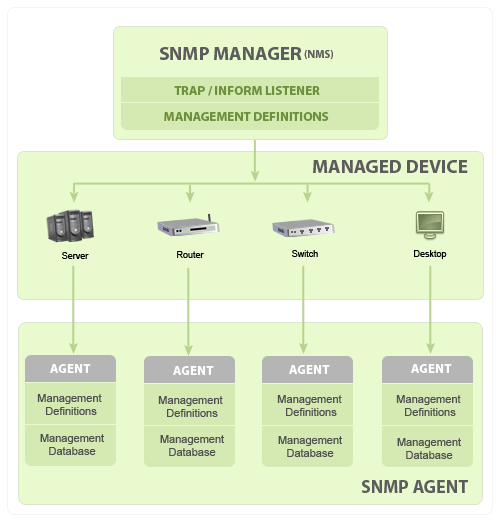
\includegraphics[width=10cm]{graphics/snmp-components}
    \caption{Diagrama básico de comunicaciones SNMP}
    \label{fig:diagrama_comunicaciones_snmp}
\end{figure}

%%%%%%%%%%%%%%%%%%%%%%%%%%%%%%%%%%%%%%%%%%%%%%%%%%%%%%%%%%%%%%%%%%%%%%%%%%%%%%%%%%%%%%%%%%%%%%%%%%%%
\subsubsection{\gls{MIB}}
La Base de Información Gestionada (\gls{MIB}) es un tipo de base de datos que contiene información
jerárquica, con estructura de árbol, de los parámetros gestionables de cada dispositivo SNMP. La
jerarquía MIB se organiza en distintos niveles que se asignan a distintas organizaciones. Los 
primeros niveles están asignados a organizaciones de normalización (ISO, CCITT, etc) mientras que 
los niveles más bajos están asignadas a organizaciones asociadas. En la Figura \ref{fig:mib_tree} 
se puede observas esta forma de organización.


Existe un gran número de MIBs definidos por organizaciones como la \gls{IETF} así como entidades
privadas y fabricantes. La base de datos más común para la gestión de equipos en Internet es la base
MIB-II definida en el \textit{RFC1213} y ampliada con la aparición de las versiones 2 y 3 de SNMP. 
Este MIB es muy importante porque es obligatorio para todos los agentes SNMP de internet y contiene
información acerca del sistema, interfaces así como aspectos de IP (incluidas las tablas de
enrutamiento).


Todos los objetos tienen un identificador único denominado OID que permiten la identificación numérica
de cualquier nodo. Por ejemplo, sirviéndonos de la Figura \ref{fig:mib_tree} podemos ver que el del
objeto \textit{iso.org.dod.internet.mgmt.mib-2.system.sysDescr} tiene el OID 1.3.6.1.2.1.1.1.

\begin{figure}[ht]
    \centering
    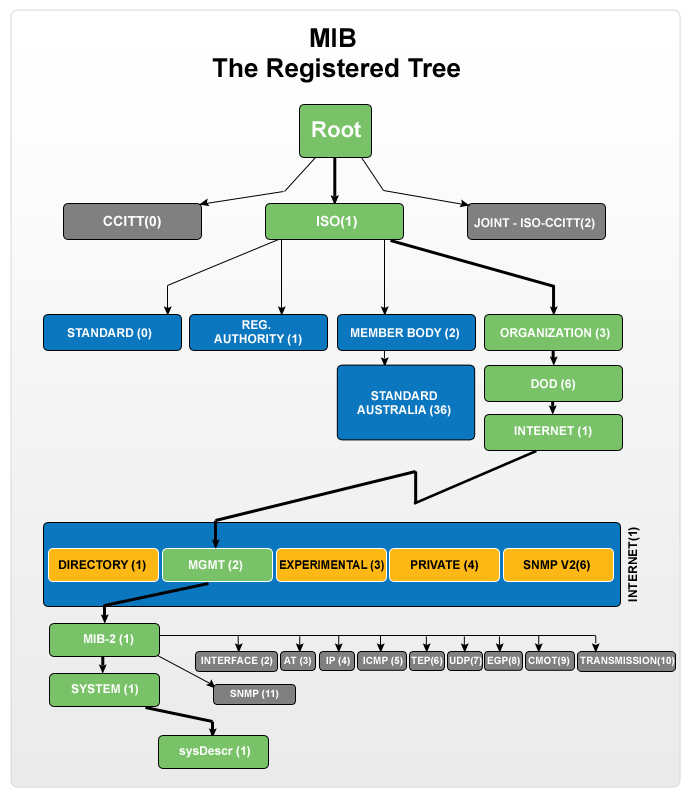
\includegraphics[width=10cm]{graphics/mib-oid-tree}
    \caption{Árbol MIB (parcial)}
    \label{fig:mib_tree}
\end{figure}

%%%%%%%%%%%%%%%%%%%%%%%%%%%%%%%%%%%%%%%%%%%%%%%%%%%%%%%%%%%%%%%%%%%%%%%%%%%%%%%%%%%%%%%%%%%%%%%%%%%%
\subsubsection{Operaciones básicas de SNMP}

Las operaciones que pueden realizar dentro del protocolo SNMP son las siguientes
\cite{mauro2005essential}:

\begin{itemize}
    \item GET: La operación GET es una petición enviada por un gestor a un agente para obtener uno o
    más valores del agente. Figura \ref{fig:snmp_get}
    \item GET NEXT: Esta operación es similar a GET. La principal diferencia es que GET NEXT obtiene
    el valor del siguiente OID del árbol MIB.
    \item GET BULK (SNMPv2 y v3): Operación usada para obtener grandes volúmenes de datos desde tablas
    MIB grandes.Figura \ref{fig:snmp_bulk}
    \item SET: Esta operación es usada por los gestores para modificar o asignar un valor dentro de un
    agente.Figura \ref{fig:snmp_set}
    \item TRAPS: Los TRAPS son señales enviadas por los agentes para notificar a los gestores de algún
    evento.Figura \ref{fig:snmp_trap}
    \item INFORM: similar a una TRAP, pero a diferencia de este INFORM incluye la confirmación por
    parte del gestor \gls{SNMP} de la recepción del mensaje
    \item RESPONSE: este es el comando usado para devolver valores a los gestores SNMP.
\end{itemize}

\begin{figure}
    \centering
    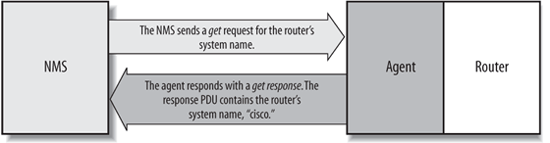
\includegraphics[width=.5\linewidth]{graphics/snmp_get}
    \caption{SNMP Get Sequence}
    \label{fig:snmp_get}
\end{figure}

\begin{figure}
    \centering
    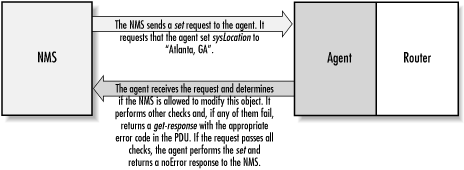
\includegraphics[width=.5\linewidth]{graphics/snmp_set}
    \caption{SNMP Set Sequence}
    \label{fig:snmp_set}
\end{figure}

\begin{figure}
    \centering
    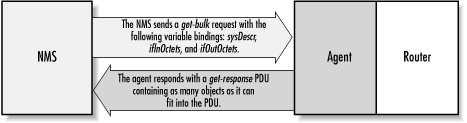
\includegraphics[width=.5\linewidth]{graphics/snmp_get_bulk}
    \caption{SNMP Get Bulk Sequence}
    \label{fig:snmp_bulk}
\end{figure}

\begin{figure}
    \centering
    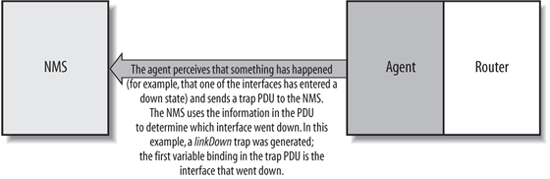
\includegraphics[width=.5\linewidth]{graphics/snmp_trap}
    \caption{SNMP Trap Sequence}
    \label{fig:snmp_trap}
\end{figure}

\subsection{Network Configuration Protocol\label{sec:NETCONF}}
El protocolo \gls{NETCONF} es un protocolo de gestión de redes desarrollado y estandarizado por la \gls{IETF}. Fue desarrollado en el grupo de trabajo NETCONF publicado en diciembre de 2006 en el \rfclink{RFC4741} y posteriormente revisado en junio 2011 en el \rfclink{RFC6241}. 

\gls{NETCONF} proporciona los mecanispos para instalar, manipular y borrar la configuración de dispositivos de red. Las operaciones del protocolo \gls{NETCONF} se realizan mediante \glspl{RPC} y usan una codificación \gls{XML} tanto para los datos que constituyen la configuración como para los mensajes del propio protocolo. 

El protocolo se puede dividir conceptualmente en cuatro capas que se pueden ver en la Figura \ref{fig:capas_netconf}:
\begin{itemize}
    \item \textbf{Transporte}: La capa de transporte proporciona un canal de comunicación entre el cliente y el servidor.
    \item \textbf{Mensajes}: La capa de mensajes proporciona una forma simple, para enmarcar y codificar los mensajes del protocolo.
    \item \textbf{Operaciones}: La capa de operaciones define el conjunto de operaciones básicas y sus parámetros.
    \item \textbf{Contenido}: Define la organización y el modelado de los datos de configuración.
\end{itemize}

\begin{figure}
    \centering
    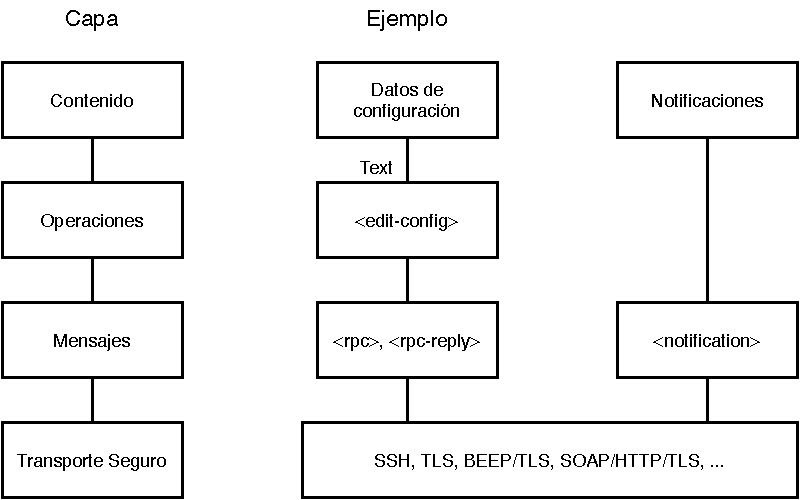
\includegraphics[scale=.75]{graphics/Capas_Netconf.pdf}
    \caption{Capas del protocolo \gls{NETCONF}}
    \label{fig:capas_netconf}
\end{figure}

\subsubsection{Transporte}

\gls{NETCONF} usa mensajes \glspl{RPC} para comunicarse. Un cliente manda una serie de solicitudes \gls{RPC} que provocan el el servidor responda con una serie de respuestas RPC. \gls{NETCONF} puede usar cualquier protocolo de transporte siempre que este proporcione la funcionalidad necesaria:

\begin{itemize}
    \item \textbf{Orientado a conexión}: \gls{NETCONF} requiere una conexión persistente entre pares.
    \item \textbf{Autenticación, Integridad y Confidencialidad}
\end{itemize}

Aunque existe soporte para muchos protocolos de transporte, los más usados son \gls{NETCONF} sobre \gls{SSH} \rfclink{RFC6242}\cite{RFC6242} y \gls{NETCONF} sobre \gls{TLS} con Autenticación mutua usando certificados X.509 \rfclink{RFC7589}\cite{RFC7589}.

\subsubsection{Mensajes}
La base del protocolo \gls{NETCONF} proporciona tres tipos de mensajes:

\begin{itemize}
    \item Solicitudes \gls{RPC} (mensajes <rpc>)
    \item Respuestas \gls{RPC} (mensajes <rpc-reply>)
    \item Notificaciones de eventos (mensajes <notification>)
\end{itemize}

Cada mensaje del protocolo \gls{NETCONF} es un documento \gls{XML} bien formado y codificado usando UTF-8. Las solicitudes y las respuestas se relacionan entre si mediante un atributo \enquote{message-id} de forma que el protocolo \gls{NETCONF} permite el \enquote{pipelining} de mensajes.

\subsubsection{Operaciones}

El protocolo \gls{NETCONF} proporciona un conjunto pequeño de operaciones de bajo nivel para gestionar la configuración de los dispositivos y recuperar información de estado. El protocolo base proporciona operaciones para recuperar, configurar, copiar y borrar elementos de configuración. Otras operaciones se pueden añadir en función de las capacidades anunciadas por el dispositivo. Las operaciones básicas son:

\begin{itemize}
    \item \textbf{get}: Recupera la configuración y la información de estado del dispositivo. A diferencia de \enquote{get-config} también puede recuperar información de estado.
    \item \textbf{get-config}: Recupera todo o parte de un datastore de configuración especifico. 
    \item \textbf{edit-config}: Carga todo o parte de una configuración a un datastore especifico.
    \item \textbf{copy-config}: Crea o reemplaza un datastore completo con los contenidos de otro datastore.
    \item \textbf{delete-config}: Elimina un datastore de configuración. El almacén de datos \enquote{running} no puede ser eliminado.
    \item \textbf{lock}: Permite a un cliente bloquear temporalmente un almacén de datos con el fin de realizar cambios sin interacciones por parte de otros clientes \gls{NETCONF}.
    \item \textbf{unlock}: Libera el bloqueo iniciado por una operación \enquote{lock} permitiendo de nuevo realizar modificaciones sobre el datastore afectado.
    \item \textbf{close-session}: Solicita la finalización de forma elegante de una sesión de \gls{NETCONF}.
    \item \textbf{kill-session}: Fuerza la finalización de una sesión \gls{NETCONF}
\end{itemize}

\subsubsection{Contenido}

La última revisión del protocolo \gls{NETCONF}, el \rfclink{RFC6241}\cite{RFC6241} no proporciona una definición para la capa de Contenido, quedando fuera del alcance de dicho documento. Los datos de configuración se definen mediante el lenguaje de modelado de datos YANG que se explicará en la Sección \ref{sec:yang_data_model}.





\subsection{Google Network Management Interface\label{sec:gNMI}}

\section{Yang Data Model}

\subsection{Introducción al modelado YANG}

\subsection{OpenConfig modelos}

\section{Telemetría}

\subsection{Framework}

Resumen de
https://tools.ietf.org/id/draft-opsawg-ntf-00.html

\subsection{Network Configuration Notifications\label{sec:NETCONFNot}}

https://tools.ietf.org/html/rfc5277

\subsection{YANG Push Notifications\label{sec:YANGNot}}

https://datatracker.ietf.org/doc/rfc8641/
https://tools.ietf.org/id/draft-ietf-netconf-notification-capabilities-05.html

\clearpage
%
% Diseño
%
\chapter{Diseño\label{sec:disenho}}

\section{Base de datos}

Para poder implementar los servicios de notificaciones push es necesaria una forma de acceder a los
datos que se solicitan en las peticiones de tipo \textit{establish-subscription}. El sistema que 
proporcione estos datos debe cumplir varias condiciones:

\begin{enumerate}
    \item Primero, debe ser capaz de almacenar los datos siguiendo el esquema YANG correspondiente. 
    El lenguaje YANG define una estructura de datos en forma de árbol, definiendo la jerarquía entre
    objetos y pudiéndose codificar en diferentes lenguajes como pueden ser \gls{XML} o \gls{JSON}.
    Por ejemplo el siguiente modelo YANG ~\ref{lst:ejemplo-yang} se corresponde a los datos \gls{XML}
    listados en el Código \ref{lst:ejemplo-instancia-yang}:
    
    \lstinputlisting[label={lst:ejemplo-yang}, 
                        frame=single,
                        caption=Ejemplo de modelo YANG]
                        {src/code_snippets/ejemplo_yang_1.txt}
                        
    \lstinputlisting[label={lst:ejemplo-instancia-yang},
                        language=XML, 
                        frame=single,
                        caption=Una posible instancia del modelo YANG anterior]
                        {src/code_snippets/ejemplo_intancia_yang.xml}

    \item Debe ser compatible con, al menos, el lenguaje de programación utilizado, en este caso,
    Python 3.x, aunque es preferible que exista soporte para otros lenguajes.
    
    \item Debe proporcionar algún mecanismo de notificación de cambios de los datos para poder
    proporcionar notificaciones de tipo \textit{on-change} sin necesidad de hacer \textit{pooling}.
\end{enumerate}

En base a los criterios anteriores se han elegido tres bases de datos candidatas: MongoDB,
Prometheus y Redis. A continuación se van a evaluar cada una de ellas con el fin de elegir la base de datos más adecuada para el proyecto. En el Anexo \ref{appendix:bases_de_datos} se adjunta una tabla comparativa de los tres sistemas.

\subsection{MongoDB}
MongoDB es una base de datos multiplataforma orientada a documentos, clasificada como una base de 
datos NoSQL, que usa el lenguaje BSON, muy similar a JSON en vez del modelo tradicional de las 
bases de datos relacionales donde los datos se almacenan en filas. 

Como podemos ver en la figura~\ref{fig:Mongo_vs_RDBMS}, las tablas se corresponden a colecciones,
las filas se corresponden a documentos y las columnas se corresponden a campos de los documentos
pero con la ventaja de que MongoDB usa un modelo \textit{schemaless}, por tanto, los campos de los
documentos no son fijos. Dentro de una misma colección cada documento puede tener diferentes campos,
permitiendo la modificación de la estructura de un documento sin tener restricciones impuestas por
la colección (en un RDBMS todas las filas tienen las mismas columnas, es menos flexible). 

% TODO: añadir imágen  de objetos distintos en la misma colección emulando uno de los modelos yang.

\begin{figure}
    \centering
    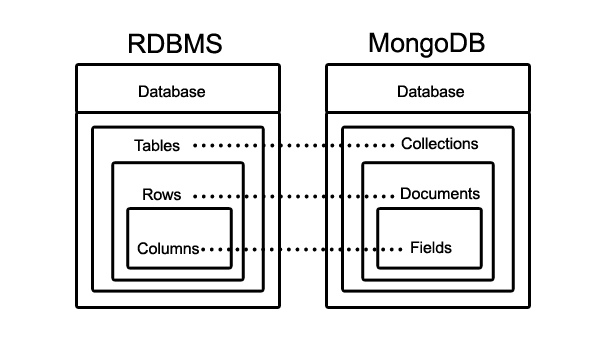
\includegraphics[width=10cm]{graphics/MongoDB_vs_RMSBD}
    \caption{Equivalencias entre MongoDB y RDBMS}
    \label{fig:Mongo_vs_RDBMS}
\end{figure}

Como ya hemos visto en la introducción de este apéndice, al ser capaz de guardar datos con una
estructura \gls{JSON} es muy idoneo para este proyecto. Además es compatible con muchos lenguajes de
programación como C, CSharp, C++, Go, Java, Javascript, PHP y \textbf{Python}.
\subsection{Prometheus}
Prometheus \cite{prometheus} es una aplicación open-source usada para la monitorización de 
eventos y envío de alertas en tiempo real. Usa base de datos orientada a series temporales, 
dónde cada serie se identifica por un nombre, P.E \enquote{Used Bandwidth \%}, y un conjunto 
de pares clave-valor. Además, cuenta con un potente lenguaje de consultas llamado PromQL que
permite la manipulación de series temporales para la generación de gráficos, tablas y alertas.

Desgraciadamente, este sistema no cumple con varios de nuestros requisitos. En primer lugar,
está optimizado para series temporales mientras que para este proyecto se necesita guardar
instancias de modelos YANG. En segundo lugar, aunque Prometheus dispone de un sistema de alertas
llamado \textit{alertmanager} los tipos de notificaciones de proporciona no se corresponde con las 
necesidades del proyecto. Tal como se ha explicado al principio de esta sección, se necesita un 
mecanismo que detecte cambios en las instancias de los modelos YANG soportados y notificar el 
hilo/proceso que estuviese monitorizando un subárboles determinado de un modelo YANG. Sin embargo,
el \textit{alertmanager} lo que proporciona son alertas basadas en eventos (P.E Temperatura de la 
CPU > 90º durante más de 2 minutos) para administradores de sistemas, ofreciendo diferentes canales
como Slack, Telegram, Correo, SMS, etc. 


\begin{figure}
    \centering
    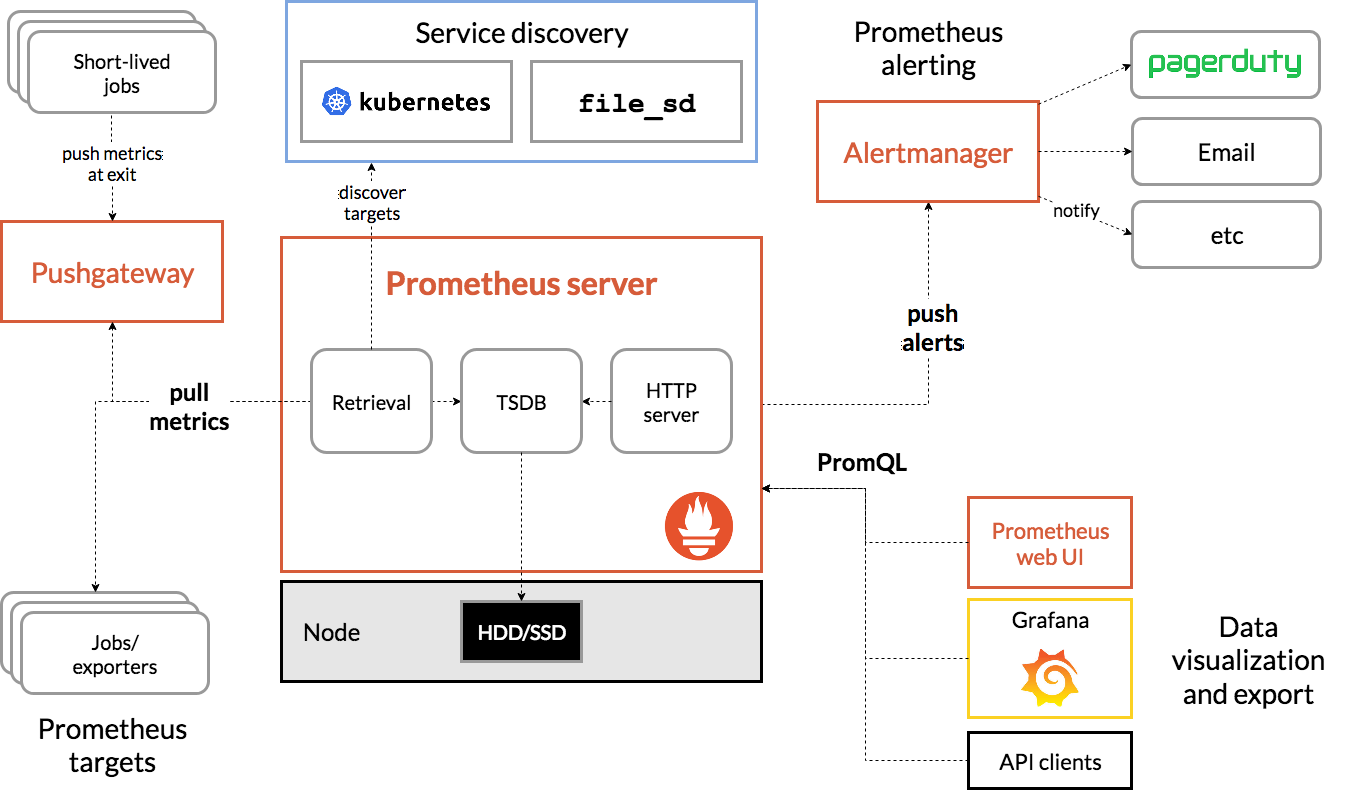
\includegraphics[width=15cm]{graphics/prometheus_architecture.png}
    \caption{Arquitectura de Prometheus}
    \label{fig:prometheus_estructura}
\end{figure}

Sin embargo, aunque no sea un sistema adecuado para almacenar los datos de un datastore YANG, se podría estudiar la utilización de Prometheus como sistema de visualización de series temporales que recibiría el cliente a través de notificaciones NETCONF, P.E. el cliente se podría subscribir para recibir la temperatura de la CPU cada 0.5 segundos y se podría utilizar Prometheus para almacenar esa serie temporal y usar sus herramientas de visualización para interpretar los datos 



\subsection{Redis} 
Redsis \cite{redsis_main_page} es un sistema de almacenamiento de datos en memoria de código abierto (licencia BSD) que se utiliza como base de datos, caché y como sistema de envío de mensajes. Admite estructuras de datos como cadenas, hashes, listas, conjuntos, conjuntos ordenados, mapas de bits, indices geoespaciales y flujos. Redis tiene replicación integrada, soporta scripting LUA, transacciones y distintos niveles de persistencia en disco. 

Redis guarda los datos en una estructura de tipo Hashtable como pares clave-valor soportando todos los
tipos de datos ya mencionados. Sin embargo, no permite la existencia de objetos anidados y por tanto no es capaz de representar un objeto YANG de forma completa (solo podría representar un solo nivel).
Además, no existe soporte para la mayoría de tipos de datos que podemos encontrar en las hojas de un modelo YANG como Integer16/32/64, Float y Double.

Redis tiene un sistema de alertas/notificaciones llamado Redis Keyspace Notifications que permite
a clientes subscribirse a canales para recibir notificaciones de eventos que afectan los datos de Redis. 

Sin embargo, debido a las limitaciones de este tipo de almacenamiento, considero que el sistema no es adecuado.

\begin{figure}
    \centering
    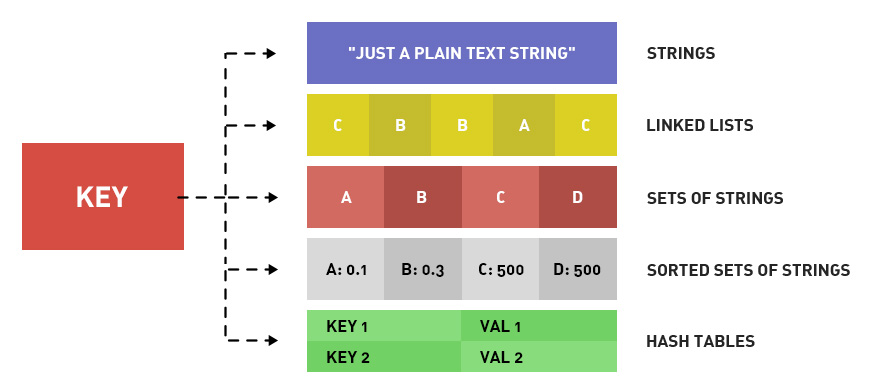
\includegraphics[width=15cm]{graphics/redis-data-structure-types.jpeg}
    \caption{Estructura de Datos de Redis}
    \label{fig:redis_estructura}
\end{figure}

\subsection{Decisión de diseño}





\section{Virtualizacion}
  \subsection{Maquinas Virtuales}
  \subsection{Docker}
  \subsection{Kubernetes}
\subsection{Decisión de diseño}

% \begin{figure}
%     \centering
%     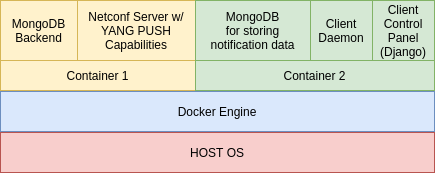
\includegraphics{graphics/docker.png}
%     \caption{Caption}
%     \label{fig:my_label}
% \end{figure}

\clearpage
%
% Desarrollo
%
\chapter{Desarrollo\label{sec:desarrollo}}

TODO: Desarrollo del proyecto
Test mod
\clearpage
%
% Resultados
%
\chapter{Resultados\label{sec:resultados}}
\Large{INCOMPLETO.}
\section{Entorno de pruebas}

\section{Validación del protocolo YANG Push}

\subsection{Subscripciones periódicas}
\Large{INCOMPLETO.}

\subsubsection{Period interval}

\paragraph{Flujo de trabajo}

diagrama de websequence

\paragraph{Intercambio de mensajes}


\subsubsection{Anchor-Time}

\paragraph{Flujo de trabajo}

diagrama de websequence

\paragraph{Intercambio de mensajes}



\subsection{Subscripciones sobre cambios}

dampening-period
change-type
sync-on-start (prioridad baja si da tiempo)

TODO: Pruebas y resultados

\subsection{Xpath}

\subsection{Performance}


\clearpage
%
% Conclusiones
%
\chapter{Conclusiones y trabajo futuro\label{sec:conclusiones}}

\section{Conclusiones}
TODO: Conclusiones sobre el trabajo realizado

\section{Trabajo futuro} 
\clearpage
%
% Página en blanco
%
\cleardoublepage

%
% Bibliografía
%
\printbibliography[heading=bibintoc]

% No expandir elementos para llenar toda la página
\raggedbottom

%
% Apéndices
%
\appendix
\cleardoublepage
\addappheadtotoc
\appendixpage

% Apéndices del TFG
\chapter{Tabla comparativa bases de datos\label{appendix:bases_de_datos}}

Para obtener información de forma más rápida y poder comparar fácilmente las características 
de los tres sistemas se ha usado el portal \href{https://db-engines.com/en/system/MongoDB\%3BPrometheus\%3BRedis}{DB-engines.com}. 
La siguiente tabla contiene las características principales de cada uno de ellos. Esta información
solo tiene carácter orientativo y será contrastada a la hora de tomar una decisión de diseño

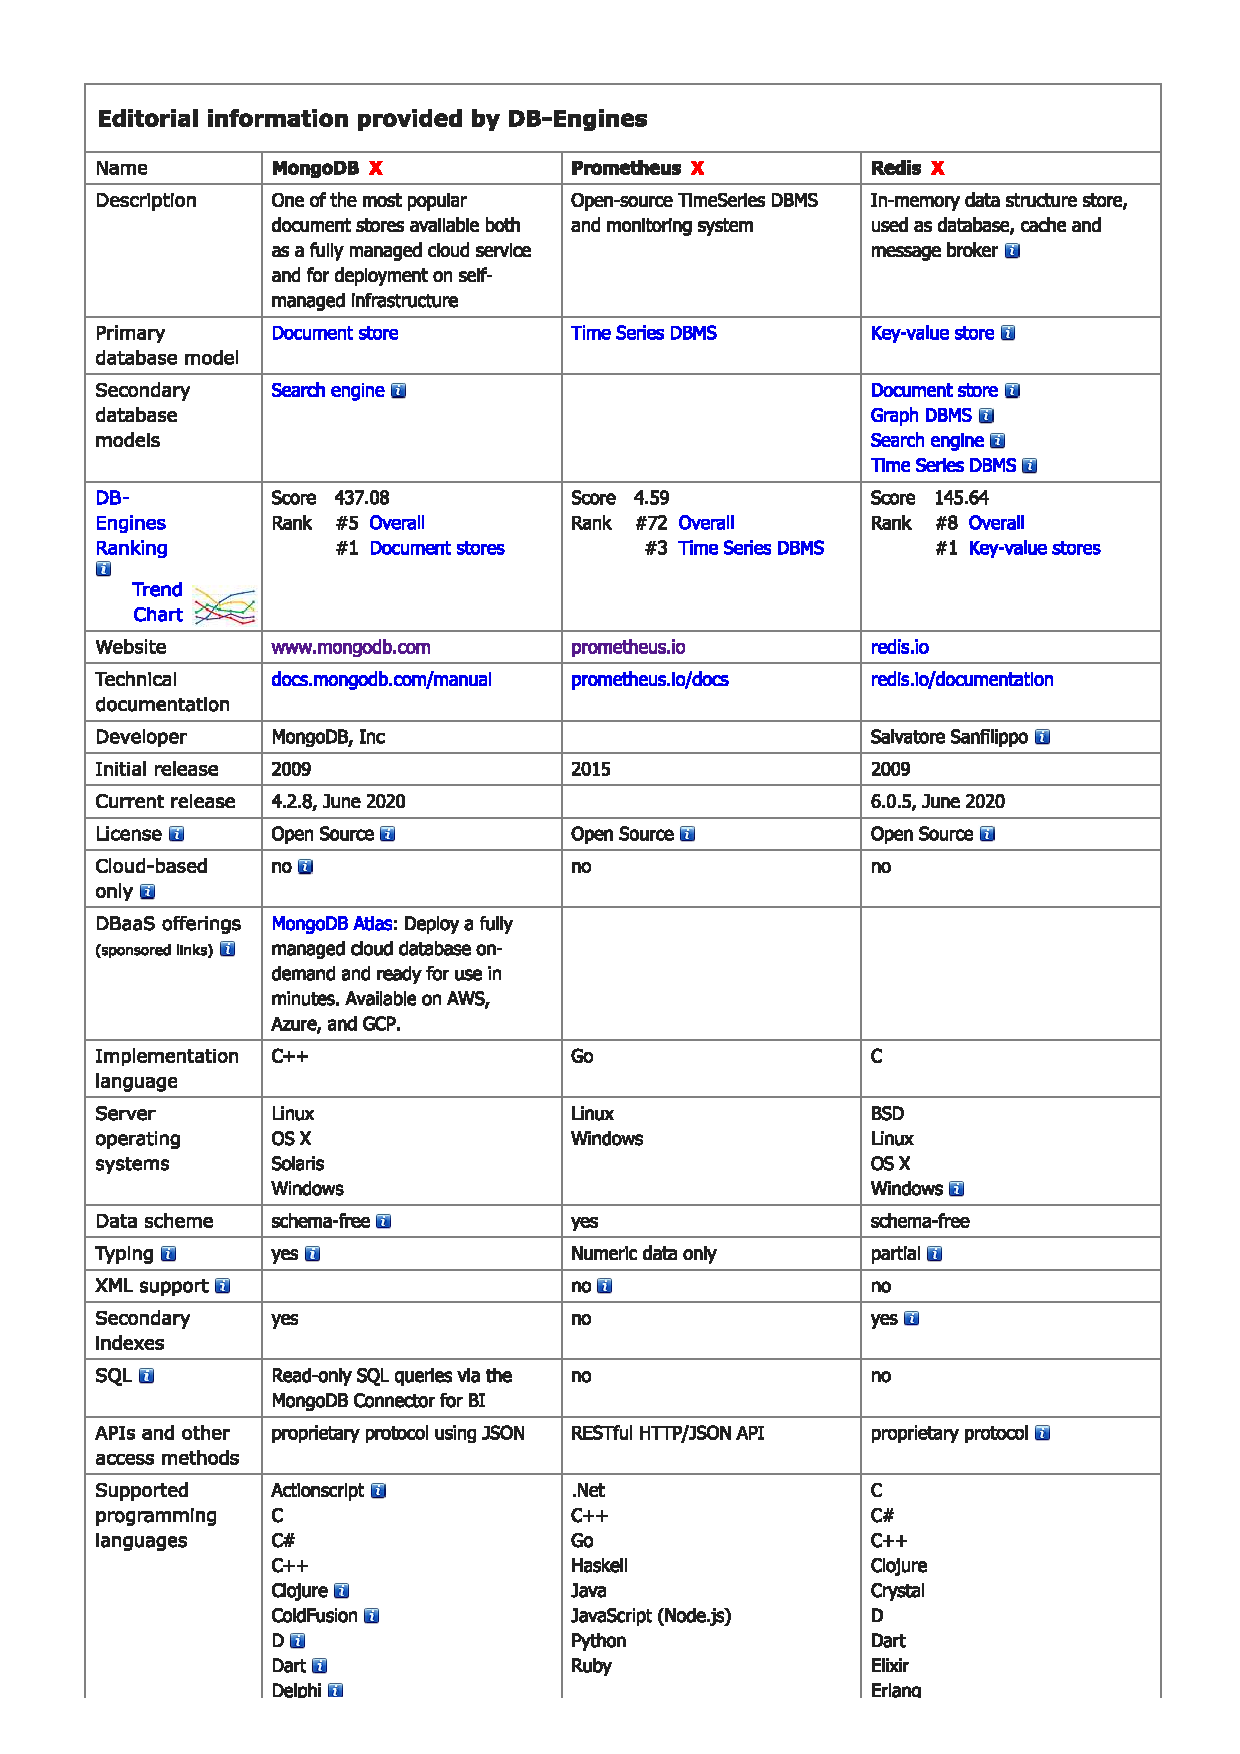
\includepdf[pages=-]{graphics/tabla_comparativa_bases_de_datos.pdf}


% Fin del documento
\end{document}
